% Asset ID: AS2ForcesTikZ-012
% Source: Chapter 5/7 Forces Transcript
% Related lesson section: Common Mistakes and Exam Traps
% Purpose: Show that friction acts opposite motion or the tendency to move.
\documentclass[tikz,border=8pt]{standalone}
\usepackage{amsmath}
\usetikzlibrary{arrows.meta, angles, quotes, decorations.pathmorphing}
\begin{document}
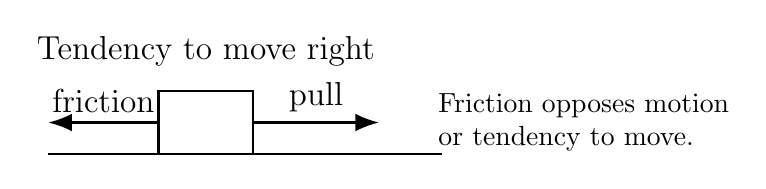
\begin{tikzpicture}[force/.style={-{Latex[length=3mm]}, thick}, comp/.style={-{Latex[length=3mm]}, thick, dashed}, label/.style={font=\large}, note/.style={font=\normalsize}]

\node[label] at (0,2.7) {Tendency to move right}; \draw[thick] (-2,1.4)--(3,1.4); \draw[thick] (-0.6,1.4) rectangle (0.6,2.2);
\draw[force] (0.6,1.8)--(2.2,1.8) node[midway,above,label] {pull}; \draw[force] (-0.6,1.8)--(-2,1.8) node[midway,above,label] {friction};
\node[note, align=left] at (4.8,1.8) {Friction opposes motion\\or tendency to move.};
\end{tikzpicture}
\end{document}
